\documentclass{beamer}
\usepackage[utf8]{inputenc}

\usetheme{Madrid}
\usecolortheme{default}
\usepackage{amsmath,amssymb,amsfonts,amsthm}
\usepackage{txfonts}
\usepackage{multicol}
\usepackage{tkz-euclide}
\usepackage{listings}
\usepackage{adjustbox}
\usepackage{array}
\usepackage{tabularx}
\usepackage{gvv}
\usepackage{lmodern}
\usepackage{circuitikz}
\usepackage{tikz}
\usepackage{graphicx}

\setbeamertemplate{page number in head/foot}[totalframenumber]

\usepackage{tcolorbox}
\tcbuselibrary{minted,breakable,xparse,skins}



\definecolor{bg}{gray}{0.95}
\DeclareTCBListing{mintedbox}{O{}m!O{}}{%
  breakable=true,
  listing engine=minted,
  listing only,
  minted language=#2,
  minted style=default,
  minted options={%
    linenos,
    gobble=0,
    breaklines=true,
    breakafter=,,
    fontsize=\small,
    numbersep=8pt,
    #1},
  boxsep=0pt,
  left skip=0pt,
  right skip=0pt,
  left=25pt,
  right=0pt,
  top=3pt,
  bottom=3pt,
  arc=5pt,
  leftrule=0pt,
  rightrule=0pt,
  bottomrule=2pt,
  toprule=2pt,
  colback=bg,
  colframe=orange!70,
  enhanced,
  overlay={%
    \begin{tcbclipinterior}
    \fill[orange!20!white] (frame.south west) rectangle ([xshift=20pt]frame.north west);
    \end{tcbclipinterior}},
  #3,
}
\lstset{
    language=C,
    basicstyle=\ttfamily\small,
    keywordstyle=\color{blue},
    stringstyle=\color{orange},
    commentstyle=\color{green!60!black},
    numbers=left,
    numberstyle=\tiny\color{gray},
    breaklines=true,
    showstringspaces=false,
}

\title{4.5.7}
\author{Aditya Mishra-EE25BTECH11005}
\date{September 30, 2025}

\begin{document}

\begin{frame}
\titlepage
\end{frame}

\begin{frame}{Question}
The equation of a line, which is parallel to $2\hat{i} + \hat{j} + 3\hat{k}$ and passes through the point $(5, -2, 4)$ is
\[
\frac{x - 5}{2} = \frac{y + 2}{-1} = \frac{z - 4}{3}.
\]
\end{frame}

\begin{frame}{Solution}
Let the point $\vec{h}$ and direction vector $\vec{m}$ be  
\[
\vec{h} = \myvec{5 \\ -2 \\ 4}, \quad 
\vec{m} = \myvec{2 \\ 1 \\ 3}.
\]

The vector equation of the line is given by
\[
\vec{x} = \vec{h} + \lambda \vec{m}, \quad \lambda \in \mathbb{R}.
\]
\end{frame}

\begin{frame}{Solution}
Expanding,  
\begin{align}
\vec{x} &= \myvec{5 \\ -2 \\ 4} + \lambda \myvec{2 \\ 1 \\ 3} \\[2mm]
           &= \myvec{5 + 2\lambda \\ -2 + \lambda \\ 4 + 3 \lambda}.
\end{align}

Hence the parametric equations of the line are  
\begin{align}
x &= 5 + 2\lambda, \\
y &= -2 + \lambda, \\
z &= 4 + 3\lambda, \quad \lambda \in \mathbb{R}.
\end{align}
\end{frame}

\begin{frame}{Solution}
Therefore, the symmetric form of the line is
\[
\boxed{\frac{x - 5}{2} = \frac{y + 2}{1} = \frac{z - 4}{3}}.
\]

Which is different from the equation in the question:
\[
\frac{x - 5}{2} = \frac{y + 2}{-1} = \frac{z - 4}{3}
\]

Hence, the statement:

	The equation of a line, which is parallel to $2\hat{i} + \hat{j} + 3\hat{k}$ and passes through the point $(5, -2, 4)$ is $\frac{x - 5}{2} = \frac{y + 2}{-1} = \frac{z - 4}{3}$ is \textbf{False}.
\end{frame}
\begin{frame}{Plot}
\begin{figure}
    \centering
    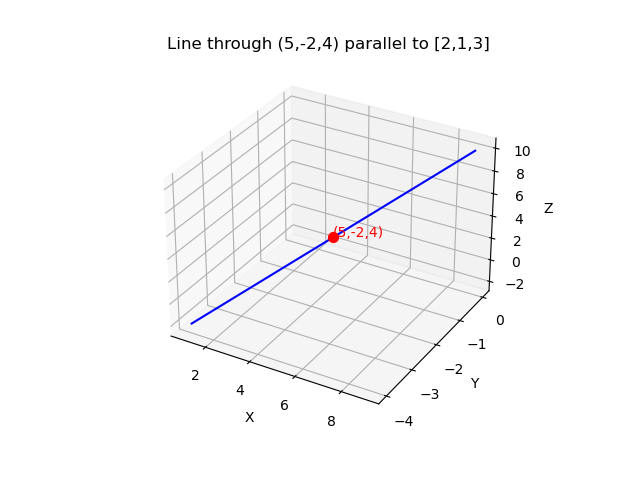
\includegraphics[width=0.8\columnwidth]{Figs/Figure.png}
\end{figure}
\end{frame}

\begin{frame}{Codes}
\centering
For Codes, refer to the URL below:  
\url{https://github.com/Aditya-Mishra11005/ee1030-2025/tree/main/ee25btech11005/matgeo/4.5.7/Codes}
\end{frame}

\end{document}


